%%% The main file. It contains definitions of basic parameters and includes all other parts.

%% Settings for single-side (simplex) printing
% Margins: left 40mm, right 25mm, top and bottom 25mm
% (but beware, LaTeX adds 1in implicitly)
\documentclass[12pt,a4paper]{report}
\setlength\textwidth{145mm}
\setlength\textheight{247mm}
\setlength\oddsidemargin{15mm}
\setlength\evensidemargin{15mm}
\setlength\topmargin{0mm}
\setlength\headsep{0mm}
\setlength\headheight{0mm}
% \openright makes the following text appear on a right-hand page
\let\openright=\clearpage

%% Settings for two-sided (duplex) printing
% \documentclass[12pt,a4paper,twoside,openright]{report}
% \setlength\textwidth{145mm}
% \setlength\textheight{247mm}
% \setlength\oddsidemargin{14.2mm}
% \setlength\evensidemargin{0mm}
% \setlength\topmargin{0mm}
% \setlength\headsep{0mm}
% \setlength\headheight{0mm}
% \let\openright=\cleardoublepage

%% Character encoding: usually latin2, cp1250 or utf8:
\usepackage[utf8]{inputenc}

%% Further useful packages (included in most LaTeX distributions)
\usepackage{amsmath}        % extensions for typesetting of math
\usepackage{amsfonts}       % math fonts
\usepackage{amsthm}         % theorems, definitions, etc.
\usepackage{bbding}         % various symbols (squares, asterisks, scissors, ...)
\usepackage{bm}             % boldface symbols (\bm)
\usepackage{graphicx}       % embedding of pictures
\usepackage{fancyvrb}       % improved verbatim environment
\usepackage{natbib}         % citation style AUTHOR (YEAR), or AUTHOR [NUMBER]
\usepackage[nottoc]{tocbibind} % makes sure that bibliography and the lists
			    % of figures/tables are included in the table
			    % of contents
\usepackage{dcolumn}        % improved alignment of table columns
\usepackage{booktabs}       % improved horizontal lines in tables
\usepackage{paralist}       % improved enumerate and itemize
\usepackage[usenames]{xcolor}  % typesetting in color

\usepackage{todonotes}
%%% Basic information on the thesis

% Thesis title in English (exactly as in the formal assignment)
\def\ThesisTitle{Graph Based SLAM on NDT Maps}

% Author of the thesis
\def\ThesisAuthor{Lukáš Jelínek}

% Year when the thesis is submitted
\def\YearSubmitted{2015}

% Name of the department or institute, where the work was officially assigned
% (according to the Organizational Structure of MFF UK in English,
% or a full name of a department outside MFF)
\def\Department{Name of the department}

% Is it a department (katedra), or an institute (ústav)?
\def\DeptType{Department}

% Thesis supervisor: name, surname and titles
\def\Supervisor{Supervisor's Name}

% Supervisor's department (again according to Organizational structure of MFF)
\def\SupervisorsDepartment{department}

% Study programme and specialization
\def\StudyProgramme{study programme}
\def\StudyBranch{study branch}

% An optional dedication: you can thank whomever you wish (your supervisor,
% consultant, a person who lent the software, etc.)
\def\Dedication{%
Dedication.
}

% Abstract (recommended length around 80-200 words; this is not a copy of your thesis assignment!)
\def\Abstract{%
Abstract.
}

% 3 to 5 keywords (recommended), each enclosed in curly braces
\def\Keywords{%
{key} {words}
}

%% The hyperref package for clickable links in PDF and also for storing
%% metadata to PDF (including the table of contents).
\usepackage[pdftex,unicode]{hyperref}   % Must follow all other packages
\hypersetup{breaklinks=true}
\hypersetup{pdftitle={\ThesisTitle}}
\hypersetup{pdfauthor={\ThesisAuthor}}
\hypersetup{pdfkeywords=\Keywords}
\hypersetup{urlcolor=blue}

% Definitions of macros (see description inside)
%%% This file contains definitions of various useful macros and environments %%%
%%% Please add more macros here instead of cluttering other files with them. %%%

%%% Minor tweaks of style

% These macros employ a little dirty trick to convince LaTeX to typeset
% chapter headings sanely, without lots of empty space above them.
% Feel free to ignore.
\makeatletter
\def\@makechapterhead#1{
  {\parindent \z@ \raggedright \normalfont
   \Huge\bfseries \thechapter. #1
   \par\nobreak
   \vskip 20\p@
}}
\def\@makeschapterhead#1{
  {\parindent \z@ \raggedright \normalfont
   \Huge\bfseries #1
   \par\nobreak
   \vskip 20\p@
}}
\makeatother

% This macro defines a chapter, which is not numbered, but is included
% in the table of contents.
\def\chapwithtoc#1{
\chapter*{#1}
\addcontentsline{toc}{chapter}{#1}
}

% Draw black "slugs" whenever a line overflows, so that we can spot it easily.
\overfullrule=1mm

%%% Macros for definitions, theorems, claims, examples, ... (requires amsthm package)

\theoremstyle{plain}
\newtheorem{thm}{Theorem}
\newtheorem{lemma}[thm]{Lemma}
\newtheorem{claim}[thm]{Claim}

\theoremstyle{plain}
\newtheorem{defn}{Definition}

\theoremstyle{remark}
\newtheorem*{cor}{Corollary}
\newtheorem*{rem}{Remark}
\newtheorem*{example}{Example}

%%% An environment for proofs

%%% FIXME %%% \newenvironment{proof}{
%%% FIXME %%%   \par\medskip\noindent
%%% FIXME %%%   \textit{Proof}.
%%% FIXME %%% }{
%%% FIXME %%% \newline
%%% FIXME %%% \rightline{$\square$}  % or \SquareCastShadowBottomRight from bbding package
%%% FIXME %%% }

%%% An environment for typesetting of program code and input/output
%%% of programs. (Requires the fancyvrb package -- fancy verbatim.)

\DefineVerbatimEnvironment{code}{Verbatim}{fontsize=\small, frame=single}

%%% The field of all real and natural numbers
\newcommand{\R}{\mathbb{R}}
\newcommand{\N}{\mathbb{N}}

%%% Useful operators for statistics and probability
\DeclareMathOperator{\pr}{\textsf{P}}
\DeclareMathOperator{\E}{\textsf{E}\,}
\DeclareMathOperator{\var}{\textrm{var}}
\DeclareMathOperator{\sd}{\textrm{sd}}

%%% Transposition of a vector/matrix
\newcommand{\T}[1]{#1^\top}

%%% Various math goodies
\newcommand{\goto}{\rightarrow}
\newcommand{\gotop}{\stackrel{P}{\longrightarrow}}
\newcommand{\maon}[1]{o(n^{#1})}
\newcommand{\abs}[1]{\left|{#1}\right|}
\newcommand{\dint}{\int_0^\tau\!\!\int_0^\tau}
\newcommand{\isqr}[1]{\frac{1}{\sqrt{#1}}}

%%% Various table goodies
\newcommand{\pulrad}[1]{\raisebox{1.5ex}[0pt]{#1}}
\newcommand{\mc}[1]{\multicolumn{1}{c}{#1}}


% Title page and various mandatory informational pages
\begin{document}
%%% Title page of the thesis and other mandatory pages

%%% Title page of the thesis

\pagestyle{empty}
\hypersetup{pageanchor=false}
\begin{center}

\centerline{\mbox{
\includegraphics[width=166mm]{../img/logo-en.pdf}}}

\vspace{-8mm}
\vfill

{\bf\Large BACHELOR THESIS}

\vfill

{\LARGE\ThesisAuthor}

\vspace{15mm}

{\LARGE\bfseries\ThesisTitle}

\vfill

\Department

\vfill

\begin{tabular}{rl}

Supervisor of the bachelor thesis: & \Supervisor \\
\noalign{\vspace{2mm}}
Study programme: & \StudyProgramme \\
\noalign{\vspace{2mm}}
Study branch: & \StudyBranch \\
\end{tabular}

\vfill

% Zde doplňte rok
Prague \YearSubmitted

\end{center}

\newpage

%%% Here should be a bound sheet included -- a signed copy of the "bachelor
%%% thesis assignment". This assignment is NOT a part of the electronic
%%% version of the thesis. DO NOT SCAN.

%%% A page with a solemn declaration to the bachelor thesis

\openright
\hypersetup{pageanchor=true}
\pagestyle{plain}
\pagenumbering{roman}
\vglue 0pt plus 1fill

\noindent
I declare that I carried out this bachelor thesis independently, and only with the cited
sources, literature and other professional sources.

\medskip\noindent
I understand that my work relates to the rights and obligations under the Act No.~121/2000 Sb.,
the Copyright Act, as amended, in particular the fact that the Charles
University has the right to conclude a license agreement on the use of this
work as a school work pursuant to Section 60 subsection 1 of the Copyright Act.

\vspace{10mm}

\hbox{\hbox to 0.5\hsize{%
In ........ date ............	% FIXME!
\hss}\hbox to 0.5\hsize{%
signature of the author
\hss}}

\vspace{20mm}
\newpage

%%% Mandatory information page of the thesis

\openright

\vbox to 0.5\vsize{
\setlength\parindent{0mm}
\setlength\parskip{5mm}

Title:
\ThesisTitle

Author:
\ThesisAuthor

\DeptType:
\Department

Supervisor:
\Supervisor, \SupervisorsDepartment

Abstract:
\Abstract

Keywords:
\Keywords

\vss}

\newpage

%%% Dedication

\openright

\noindent
\Dedication

\newpage

\openright
\pagestyle{plain}
\pagenumbering{arabic}
\setcounter{page}{1}

%%% A page with automatically generated table of contents of the bachelor thesis

\tableofcontents

%%% Each chapter is kept in a separate file
\chapter*{Introduction}
\addcontentsline{toc}{chapter}{Introduction}
Humanity has envisioned many tasks which could be carried out by robots including transportation, health care, save and rescue and many more. Robots of current world can efficiently operate only in very limited conditions. To solve problems of the future we need fast and reliable algorithms for our robots. Big question in field of mobile robotics is how to efficiently localize robot and create map as precise as possible. This problem is often referred to as \gls{SLAM} problem.

Good localization is crucial part of any good navigation software. Generated map plays important role in path planning and  multi-robot coordination. SLAM algorithm should relay mostly on robots internal sensors like, e.g., sonars, cameras, wheel encoders. Using \gls{GPS} is only possible in outdoor environment. Precision of this localization is very often not good enough to successfully navigate robot.

In last decade many high quality \gls{SLAM} algorithms where presented. Solution to full problem of map building and robot positioning is usually done by combining algorithms for map representation, sensor measurement registration and position estimation. This work solves full \gls{SLAM} problem by combination of \gls{NDT} map building process and scan registration with well developed research branch of graph-based \gls{SLAM} optimizing engines. To achieve this combination this work presents extended implementation of \gls{NDT} mapping process and new way of robust scan-matching on \gls{NDT} map. Implementation is done in \gls{ROS} to make it easy to test, use and improve.

This text is structured as follows: Key algorithms and concepts used in whole problem solution are explained in Section 1. In Section 2, is described process of scan matching, graph building, optimization and NDT mapping. Section 3 presents implementation details of this algorithm. Section 4 discuss mapping results and comparison to well known implementations in ROS.  
\todo{fix me}


\chapter{Used algorithms and key concepts}
This section offers basing introduction to multiple state-of-the-art algorithms used in this work. Good understanding of these concepts is crucial for full comprehension of section 3 \todo{ref}. 

\section{SLAM problem definition}
Successfully solving \gls{SLAM} problem means to find location of robot in every time step and be able to create map at that time-stamp. In real world we deal with robot's sensors which have always some inherited noise. This means we are not able to fully say exact position of robot. This is main reason why to use probabilistic definition of problem. Robot moves through unknown space along trajectory expressed as variables $ \textbf{x}_{1:T} = \{\textbf{x}_{1},...,\textbf{x}_{T}\} $. While moving robot is taking odometry measurements $ \textbf{u}_{1:T} = \{\textbf{u}_{1},...,\textbf{u}_{T}\}$ and perception of environment $ \textbf{z}_{1:T} = \{\textbf{z}_{1},...,\textbf{z}_{T}\}$ Solving SLAM than means finding out probability of the robot's trajectory $ \textbf{x}_{1:T}$ and a map \textbf{m} of local environment given all the measurements and initial pose $ \textbf{x}_{0}$:
\begin{equation}
p(\textbf{x}_{1:T}, \textbf{m}\: |\:  \textbf{z}_{1:T}, \textbf{u}_{1:T}, \textbf{x}_{0})
\end{equation}
Odometry is usually acquired by robots wheel encoders or by incremental scan-matching. Odometry is represented in 2D by triple $(x,y,\theta)$ or by three dimensional transformation matrix. Perceptions of environment might come from different sources. In this work we expect distance measurements from laser scanner or kinect sensor. Initial pose can be interpreted as origin of coordinate system for global map. Representation of the map is more described in section \ref{MAP_REPRE}.

\subsection{SLAM categories}
\newpage
\subsection{Graph-based SLAM}
A graph-based SLAM solves SLAM problem by constructing graph representation of the problem. This graph is commonly called a pose graph. Nodes of the graph represent potential poses of robot at certain time stamp $ T $. Therefore, nodes are representing our trajectory $ \{\textbf{x}_{1},...,\textbf{x}_{T}\} $. Nodes also hold state of the current map. Edges in the graph represent possible spatial transformation between nodes. Edge is generated out of noisy sensor data. Therefore, we need to model uncertainty of this movement. It is represented by probability distribution and included in the edge. Generation of constrains is done by algorithm's front-end. It creates them either from odometry $  \textbf{u}_{T} $ or by measurement data  $ \textbf{z}_{T} $ registration. Once the graph is completed ,it is optimized by algorithms back-end. Result of this process is the most likely position of all nodes in the graph.

\subsection {Pose graph creation}
\label{Pose_graph_creation}
Loop closure edge generation 
\newpage

\newpage
\subsection{Optimization}
\newpage



\section{Map representation}
\label{MAP_REPRE}
Successful solving SLAM problem should output map of the unknown environment. This map needs to be stored for local path planning and obstacle avoidance. It is also needed for scan registration. Algorithms for avoiding obstacles very often need precise map. Map should keep low memory consumption, because robots very often have limited access to memory. Scan registration algorithms usually might benefit from maps with high precision.

Point-cloud is map representation which stores all measured points. This is very precise representation. All input data is still in its raw form. We are not loosing any information. Scan-matching algorithms e.g. \gls{ICP} is working on top of this datastructure. It is very easy to convert from this model to different type of map if needed. Problematic is memory consumption. If robot runs for long period with higher frequency of data production, it is likely that robot will run out of memory.

Occupancy map is grid based type. It consists of grid with cells. In every cell we have just one value describing probability that this cell is occupied. Value becomes higher with more incoming data measurements. It has constant memory consumption with respect to time of robot's run-time. It is possible to use this representation for map to map registration process. This model is also possible to represent empty spaces (low probability). This feature is used by many path planning and obstacle avoidance algorithms. That is why, occupancy maps are main output format for SLAM algorithms in ROS. It is important to select good resolution of grid. Finer grid offers better detail but higher memory consumption.

Quad-tree is a tree data structure. Each node of the tree has exactly four children. Nodes are decomposing space into sub-areas. Every node has its threshold. When it is reached, cell subdivides into four smaller cells. This process dynamically change resolution of the grid. This way we get higher precision in places where it matters more. Maximal precision is usually bounded by minimal size of leaf nodes.

\gls{NDT} representation uses grid based datastructure. Each cell has normal distribution parameters calculated based on inserted points. This model offers constant memory consumption over time. In comparison, \gls{NDT} has better representation of inner points than octree (3D case of quad-tree). This was proven as convenient by \cite{Saarinen13}. They have shown that coarser \gls{NDT} grid can have similar results in precision of space representation than finer octree map. \gls{NDT} grids have their own class of registration whoch will be explained in next sections.     
\todo{picture of occupancy grid, pointcloud ndt grid}
\newpage


\subsection{NDT grid}
\label{subsec:NDT_grid}
The normal distributions transform(NDT) grid representation was first time used by \cite{Biber03} in their scan registration process. Central idea was to convert laser scan into grid with cells containing normal distributions. Points in space from laser scanner are first separated into corresponding cells. From points in sigle cell we approximate normal distribution $(\mu_{i},P_{i})$ by calculating mean and covariance:
\begin{equation}
\mu_{i} = \dfrac{1}{n}\sum_{k=1}^{n}x_{k}
\end{equation}  
\begin{equation}
P_{i} = \dfrac{1}{n-1}\sum_{k=1}^{n}(x_{k}-\mu_{i})(x_{k}-\mu_{i})^{t}
\end{equation} 
NDT grid was than used for registration.Originally proposed grid could be updated with new laser scans only by keeping used points and recalculating all cells again. This has changed with proposed recursive covariance update step by \cite{Saarinen13}. Their update step offers way how to fuse in new measurements. First it calculate normal distributions for added points. In second step, it merges old covariances with new one.

Consider two sets of measurement $\{x_{i}\}^{m}_{i=1}$ and $\{y_{i}\}^{n}_{i=1}$ than formula for mean calculation is in equation \eqref{NDT_mean_RCU}. Recursive update for covariance (RCU) is in equation \eqref{NDT_covar_RCU}
\begin{equation}
T_{x} = \sum_{i =1}^{m}x_{i} \quad
T_{y} = \sum_{i =1}^{n}y_{i} \quad
T_{x\oplus y} = T_{x} + T_{y} 
\end{equation}

\begin{equation}
\label{NDT_mean_RCU}
\mu_{x\oplus y} =\dfrac{1}{m + n}T_{x\oplus y}
\end{equation} 

\begin{equation}
S_{x} = \sum_{i=1}^{m}(x_{i} - \frac{1}{m}T_{x})(x_{i} - \frac{1}{m}T_{x})^{T} \quad 
S_{y} = \sum_{i=1}^{n}(y_{i} - \frac{1}{n}T_{y})(y_{i} - \frac{1}{n}T_{y})^{T}
\end{equation}
\begin{equation}
S_{x\oplus y} = S_{x} + S_{y} + \dfrac{m}{n(m+n)}(\frac{n}{m}T_{x} - T_{x\oplus y})(\frac{n}{m}T_{x} - T_{x\oplus y})^{T}
\end{equation}
\begin{equation}
\label{NDT_covar_RCU}
P_{x\oplus y} = \dfrac{1}{m+n -1}S_{x\oplus y}
\end{equation}

Proof and further explanation for these equations can be found in work of \cite{Saarinen13} and later improved in \cite{Saarinen213}.

In addition to fusing in new laser measurements we can also easily generated coarser grid by merging cells from higher resolution grid to grid with lower resolution. This mechanism is useful in path planning where we can plan on coarser grid which could be faster. Also, we can use multi-level scan matching approaches, which will be discussed in next section \ref{Scan_reg}. Small disadvantage of this method is that we need to keep number of points used in every cell.

It is worth noting that in continual integration of scans calculated mean and covariance grow unboundedwith increasing number of points added. This could lead to numerical instabilities. Second problem is that cell's distribution contains measurements from all scans. This is problem in dynamic environment where some objects might disappear. These problems are solved by restricting maximal number of points in cell with parameter M
\begin{equation}
N_{x \oplus y} = 
\begin{cases}
n+m, & n+m < M \\
M, & n+m \geq M
\end{cases} 
\end{equation}
Parameter M modifies how fast we let RCU replace old measurements by new one. Small value of M makes adaptation faster and big M keeps weight of older data higher. This cause to have new data making smaller impact on result of process. 

\subsection{NDT-OM extension}
NDT grids offers good compromise between space and precision, but it lacks information about occupied space and unoccupied space. This is crucial for planning algorithms. This functionality was added to NDT by \cite{Saarinen13} and later improved by same authors in later work \cite{Saarinen213}. Every cell in NDT-OM is represented with parameters $c_{i}=\{\mu_{i}, p_{i}, N_{i},p_{i}\}$, where $\mu_{i}$ and $P_{i}$ are parameters of estimated normal distribution, $N_{i}$ is number of points in cell and $p_{i}$ is probability of the cell being occupied. 

Calculation of occupancy parameter is done by ray-tracing. Consider that we have current map $m_{x}$. We have calculated new NDT map $m_{y}$ from incoming distance measurements. Both maps needs to be in the same coordinate system. Ray-tracing starts at current robot position in map $m_{x}$. End point of ray-tracing is value of mean from one of the cells in new map $m_{y}$. Program visits every cell along the line and updates covariance. It is important to visit every cell just once. When is ray-tracing over we merge in all cells from $m_{y}$ into $m_{x}$ with RCU update rule.

The main idea in occupancy update calculation is that not all cells are occupied fully. Normal distribution usually occupies only part of the cell. A ray tracing through this cell might not intersect bounds of normal distribution at all. In order to consistently update occupancy the update value should not be a constant. Better option is to choose a function describing difference between map $m_{y}$ and $m_{x}$. This function with explanation might be found in \cite{Saarinen213}.
\todo{pridat obrazok rautracingu}


%Ray tracing line starts at point $x_{s}$ and ends in point $y_{i}$. We define our line in slope-intercept form with parameter $t \in \R $ and $l_{o}$ is a point on the line:
%\begin{equation}
%x(t) = \frac{y_{i} - x_{s}}{ \lVert y_{i} - x_{s} \lVert } \:t + l_{o}
%\end{equation}
%Given a normal distribution $N(\mu_{i}, P_{i})$ from the cell hit by ray-tracing, the likelihood along the line is defined as function:

\newpage   
\section{Scan registration}
\label{Scan_reg}
Scan registration is one of the key concepts in full SLAM solution. Algorithm can use scan matching between two scans to determine transformation. It tells how far robot moved between scans. Two scans might not offer enough information for successful registration. Imagine a robot which is standing in the corner of a room with sensor facing the wall. Scan from this robot has only information from very limited field of view and this might lead to matching errors. Therefore, it is usually necessary to combine individual scans to operate with more data.  

One of the algorithms which uses this process is called incremental scan-matching. It takes arriving scan and tries to match it against the map built from previous measurements. By doing so it can very well be used instead of robots odometry in \gls{SLAM}'s graph creation. Algorithms which are possible to work in incremental scan-matching are mentioned in sections \ref{subsec:P2D_NDT} and \ref{subsec:D2D_NDT}. Other often used approach is the \gls{ICP}, which is described in \ref{subsec:ICP}. All these algorithms use optimization methods, e.g. Newton's method. Good initial guess is needed in order to guarantee converge to the right solution. 

Another example of usage scan registration in \gls{SLAM} is for testing generated loop closures. Loop closures are created by \gls{SLAM}'s front-end as mentioned in section \ref{Pose_graph_creation}. Measurements from nodes which play role in loop closure are scan matched. By doing this we are trying to proof if two nodes are really overlapping.  The Biggest problem with this registration is that we have no valid prior information about positions of these nodes. These two scans might be perfectly aligned or they can be from completely different parts of the world. Registration needs to robustly estimate the transformation. In case of misleading closure algorithm should reject it. One scan-matcher capable of robust transformation calculation is mentioned in \ref{subsec:Corr}.  


Even robust scan-matchers can fail to correctly identify loop closures.  These registration mismatches can be divided into two categories.

The First category is local ambiguity. Good example of it is when robot moves in long corridor as seen in figure \ref{Pic_coridor} on the left. Environment does not have many distinctive features and algorithm selected one of three possible correct options.

The second category is global ambiguity. This ambiguity usually happens when algorithm do not have enough information about whole environment. Limited size of scans and environment with similar indistinguishable elements can resolve in wrong association. One example can be seen in figure \ref{Pic_coridor} on the right.   
     
 \begin{figure}
 \label{Pic_coridor}

 \end{figure}

  \todo{picture of corridor}
  \newpage
\subsection{NDT registration}
\label{subsec:P2D_NDT}
NDT registration process was first time explained by \cite{Biber03}. They have explained how to make 2D registration between older scan (target scan) and newer scan (source scan). Target scan was converted to NDT grid by technique mentioned in section \ref{subsec:NDT_grid}. Result of registration should be transformation defined in 2D:
\begin{equation}
T: 
\begin{pmatrix}
x' \\ y'
\end{pmatrix}
=
\begin{pmatrix}
\cos \theta  & -\sin \theta\\
\sin \theta & \cos \theta
\end{pmatrix}
\begin{pmatrix}
x \\ y
\end{pmatrix}
+
\begin{pmatrix}
t_{x} \\ t_{y} 
\end{pmatrix}
\end{equation}
where $ (t_{x},t_{y})^{T}$ represents translation and $\theta$ represents rotation. Transformation is used for transforming source scan. At the beginning of program parameters of transformation are initialized either by zero or from initial guess. For each point of transformed scan cost function is computed This function is defined as:
\begin{equation}
score(\textbf{p}) = \sum_{i}^{} \exp(-\frac{1}{2} ((T(x_{i},\textbf{p})- \mu_{i})^{T} P^{-1}_{i}   (T(x_{i},\textbf{p})- \mu_{i}) ) 
\end{equation}
where $\textbf{p} = (t_{x},t_{y}, \theta)$ are parameters of transformation, $N(\mu_{i},P_{i})$ are parameters of normal distribution where point $x$ is transformed by transformation $T$.Goal of the NDT scan-matching is to find parameters $\textbf{p}$ which maximize this function. This maximization problem is changed to minimization problem by searching for minimal value of -score. Newton's algorithm finds minimizing parameters in $p$ by iteratively solving equation 
\begin{equation}
 H \varDelta p = -g
\end{equation}  

Representation of hessian, gradient and all derivations might be found in work of \cite{magnusson09}. Magnusson also introduced new scaling parameters into score function in order to reject possible outliers. \gls{PDF} inside of cells of target \gls{NDT} grid may not be always from normal distribution. In practice any representation which approximates structure of the element is valid. Outliers are points far from the mean of distribution and cause unbounded growth of \gls{PDF}.

At the beginning, algorithm created discrete \gls{NDT} grid out of target scan. This introduces discretization problems. These problems are cause by points generating \gls{PDF} which are larger than their cells. In the original work of \cite{Biber03} this was solved by creating 4 target grids where each grid is translated by half of the cell size in single direction. This process made this algorithm inefficient. Introduction to multi-layer \gls{NDT} grid structure, presented by \cite{ulas20113d}, solved this problem. Multi-layer approach consists of several grids with different resolution. Grids are ordered from coarser grid to finer grid. Algorithm starts with coarse grid and estimates parameters of transformation. Calculated transformation is used as initial guess at lower level. This principle practically eliminated need for four overlapping grids. It also offered better convergence time and increase to robustness. Algorithm is able to converge when matched scans are farther away. Good configuration is 4 layers with cell sizes 2, 1, 0.5 and 0.25 meters. 

Another improvement to algorithm is usage of concept of linked cells. In practical registration very often part of the source scan lie far from any target cells. This causes only small portion of points contribute to score function. It can cause algorithm failure or just increase time of convergence. Linked cells prevent this by providing cells in target scan, which are close to the point from source scan. Implementation of this technique is possible with use of kD-tree with means of all cells as input points. Every point or source scan finds k-nearest cells and execute score calculation on them.

\begin{algorithm}
\label{alg:p2d_ndt}
    \caption{\gls{NDT} algortihms with muilti layer and linked cell enhancements}
\begin{algorithmic}[1]
 \Require source scan, target scan,  parameters $(x,y,\theta)$ of initial transformation, cell resolution for each layer
 \Function{NDTRegistration}{$scan_{s}$, $scan_{t}$, $p_{init}$,$resolutions$}
	 \State $\textbf{p} \gets p_{init}$
	 \ForAll{$res$ from $resolutions$}
		 \State $ndt_{t} \gets$createNDTGrid($res$,$scan_{t}$)
		 \Comment described in section \ref{subsec:NDT_grid}
		 \State transform each point $x_{i} \in scan_{trans}$ with $T(x_{i},\textbf{p})$
		 \State $\textbf{p} \gets$ computeSingleGrid($scan_{trans}$, $ndt_{t}$, $\textbf{p}$)
	 \EndFor
	 \State \Return calculated parameters $\textbf{p}$ of transformation
 \EndFunction
\end{algorithmic}
\end{algorithm}
\begin{algorithm}
\label{alg:p2d_ndt_single}
\caption{Computing transformation on with single target \gls{NDT} grid and source point cloud}
\begin{algorithmic}[1]
 \Require source scan, target NDT grid,  parameters $(x,y,\theta)$ of initial transformation
 \Function{computeSingleGrid}{$scan_{s}$, $ndt_{t}$,$p_{init}$}
	 \While {not converged}
		 \State $\textbf{p} \gets p_{init}$
		 \State $(score, g,H) \gets (0,0,0)$
		 \ForAll {points $x_{i} \in scan_{trans}$}
			 \State $\bar{x_{i}} \gets T(x_{i},\textbf{p})$
			 \State $cells \gets $find k-closest cells to $\bar{x_{i}} $
			 \ForAll{cells $c_{i} \in cells$}
			 \State \{based on \cite{magnusson09}\}
				 \State $(score,g,H) \gets (score,g,H)  + $ calcNewtonParameters($c_{i}$,$\bar{x_{i}}$)
			 \EndFor 
		 \EndFor
		 \State solve $H\varDelta p = - g$
		 \State $\textbf{p} \gets \textbf{p} + \varDelta p$
	 \EndWhile
	 \State \Return $\textbf{p}$
 \EndFunction
\end{algorithmic}
\end{algorithm}
         
 
\newpage
\subsection{D2D-NDT registration}
\label{subsec:D2D_NDT}
\gls{D2D}-\gls{NDT} is variant of \gls{NDT} registration algorithm proposed by \cite{Stoyanov01102012}. It is extension of original algorithm presented in section \ref{subsec:P2D_NDT}. Instead of using only one grid for target scan. This aproach uses two grids. One for source scan and second for target grid. Algorithm than minimize the sum of $L_{2}$ distances between pairs of \gls{PDF}'s from both grids. Formally, transformation between two sets of cells $X$ and $Y$ is defined as:
\begin{equation}
f(\textbf{p}) = \sum_{i = 1, j =1}^{n_{X}, n_{Y}} -d_{1}\exp\left( - \frac{d_{2}}{2}  \mu_{ij}^{T}(R^{T}P_{i}R + P_{j})^{-1} \mu_{ij} \right)
\end{equation}
\begin{equation}
\label{eq:D2D_2}
\mu_{ij} = R\mu_{i} + t - \mu_{j}
\end{equation}
where $\textbf{p} = (t_{x},t_{y},\theta)$; $X(\mu_{i},P_{i})$ and $Y(\mu_{j}, P_{j})$ are \gls{PDF}'s of individual cells in pair; a pair $(R,t)$ represents rotation matrix from parameter $\theta$ and translation vector $t=(t_{x},t_{y})$. Regulation parameters d1 and d2 are set to values $d_{1} = 1$ and $d_{2}=0.05$. Equation \ref{eq:D2D_2} represents difference in means where mean $u_{i}$ is transformed to new position.

Optimization of this function is done in similar way to \ref{subsec:P2D_NDT}  by utilizing Newtons method and solving $H\varDelta \textbf{p} = -g$. Derivations for calculation of hessian and gradient are presented in work of \cite{Stoyanov01102012}.

This algorithm is also possible to improve by iterating over multiple layers with different resolutions similar to \gls{NDT} registration in previous section.

In comparison, with \gls{NDT} registration this algorithm needs only \gls{NDT} grids for registration. Point cloud can be thrown away after successful creation of grid. This allow saving memory and efficiently represent maps in \gls{SLAM}. In addition, \gls{D2D} is almost ten times faster than standard \gls{NDT} registration on same dataset. This was proven in comparative study from \cite{NDTcomparative}. The main cause of this speed up is smaller number of calls for score calculation. In \gls{P2D}-\gls{NDT} mentioned in last section we need to calculate score for each point in source point cloud. In case of \gls{D2D} we just calculate score function for each cell of source grid. This is done by generating only pairs between cell from source grid and closest cell from target cell. Closest cell can be easily found by using kD-tree with values of target grid's means.
  
\subsection {ICP}
\label{subsec:ICP}
The iterative closest point (\gls{ICP}) algorithm was first introduced by \cite{chen92ICP} and it is still very popular method for registering point clouds. To briefly summaries algorithm: ICP iteratively refines position of two point clouds by optimizing the sum of square distances between corresponding pair of points from two clouds. This approach is usually called point-to-point registration. Class of algorithms based on \gls{ICP} has developed many modifications. Surrvey of base type of ICP algorithms and their comparison on well designed datasets is in work of \cite{pomerleau2013comparing}. 


\newpage
\subsection{Correlative scan registration}
\label{subsec:Corr}
Correlative scan registration is algorithm presented by \cite{olson2009real}. This method was developed to robustly solve registration problem. It does not require any initial guess. Therefore, it is possible to use this method for purposes of loop closure registration.

 The algorithm requires two point clouds. Target point cloud is used for generation of fast look up table filled with bit values. It is created by separating points from target cloud into individual cells. Every cell which has some points in it is marked as occupied. After this step we have a table with value 1 in cells with some points and value 0 in cells without points. In next step we add sensor noise to the table. As a function of our noise we use radially symmetric kernel. 
 \begin{equation}
 K_{i,j} = \exp\left(\frac{-1}{2}\left(\frac{\sqrt{(i r)^{2} + (j r)^{2}}}{\sigma}\right)^{2}\right) \eta
 \end{equation}
 \begin{equation}
 K =
 \begin{pmatrix}
  2 & 14 & 2\\
  14 & 100 & 14 \\
  2 & 14 & 2 
 \end{pmatrix}
 \end{equation}
 where $K_{i,j}$ is one element of kernel; $\sqrt{(i r)^{2} + (j r)^{2}}$ is euclidean distance from center of the kernel to the element $i,j$ with cell size parameter $r$. Standard deviation of sensor nose is abbreviated by $\sigma$ and $\eta$ is kernels max value.

 The Kernel overlaps over every occupied cell in the table. If value of kernel is higher than value in table. Table is updated with the kernels value. Generated smoothing can be seen in figure \ref{fig:Corr_smooth}.
 
 This algorithm is avoiding initial guess by trying all possible rotations and translations of source cloud. Every point of transformed source cloud is mapped into certain cell of look up table. The total score of transformed cloud is sum of all mapped cells scores. Algorithm usually tries rotations and translations from selected range. Transformation with the best score is the most probable transformation.
 
 This brute force process might take long time if we select small cell size to achieve good registration. To speed up this process we first need to avoid computationally expensive calculation of goniometric functions in transformation. This can be achieved by first generating all possible rotations of point cloud. For each rotation we try all translations from selected range with step size selected based on cell size of look up table.
 
 Real speed improvements offers usage of two layer architecture of look up tables. The first table has coarse resolution. This table is used for initial estimation on the whole range of selected rotations and translations. The transformations with best score are used in the second round. From every good transformation is generated search space voxel. Origin of voxel is taken from transformation. Size of voxel is cell size from coarse table. Search voxels are evaluated on look up table with fine resolution. Search space is this time limited to search voxel and initial transformation is taken from origin of voxel. The best result is our solution. By this process computation time drops rapidly as show in work of \cite{olson2009real}.     
    
\newpage
\section{NDT graph slam analyses}
\label{subsec:analyses}



\chapter{NDT graph-SLAM overview}
In this chapter we will present our solution to fulfill goals stated in our motivation. This chapter starts with complete overview of whole system. In next sections we explain how we have designed each part of the system. At the end of chapter, we present final loop of whole algorithm. 
\section{System composition}
\label{sec:Sys_arch}

Standard input of many \gls{SLAM} algorithms is odometry. In our case we do not require any prior information about robot movements. Robot position estimation is done by fast incremental scan matching. The only mandatory input is a point cloud extracted from robot's measurement. Scan matcher calculates relative transformation based on received point cloud and incremental scan matcher's map. We will refer to this map as to the moving window. It is created by merging multiple old point clouds. More details will be provided in section \ref{sec:window}.

Resulting transformation is used in the \gls{NDT} frame creation process. \gls{NDT} frame is small map which is created out of couple consecutive scans. Precise transformation is used to correctly merge these scans into single frame. This mini map is than used as a measurement information in a node of pose graph. Creating small \gls{NDT} frames solves problem measurements with small number of points. Imagine situation where robot is standing close to the corner of the room. In this scenario incoming point clouds hold only small number of points, because field of view is narrow. Similar problem arise if robot uses sensor with limited field of view e.g. Kinect. To solve it we need to integrate multiple scans to get better outline of the world. More information about world also helps to reduce chance of ambiguous loop defections \ref{Scan_reg} because larger frames have higher chance to include more unique features. Additionally, we also want to utilize advantages of \gls{NDT-OM} occupancy update rule. It is able to detect dynamic objects by ray-tracing and update map accordingly. This detection is done by merging multiple scans and re-observing same cell multiple times. More information about design choices behind \gls{NDT} frames are in section \ref{sec:NDT_frame}.

After \gls{NDT} frame generation phase, algorithms creates representing node in pose graph. Each two nodes are connected by odometry edge. Original odometry received from scan matching process was used to create \gls{NDT} frames. In our abstraction, odometry is represented by transformation between origins of consecutive frames. In the next step, pose graph generates possible loop closure edges. To do so we need to traverse a graph with use of Dijkstra projection and apply our radius based metric described in section \ref{sec:LoopClosureMetric}. 

The potential matches need to be robustly aligned. Solution to this problem is the most difficult. We need algorithm which is able to perform 10s of registration per second. At the same time it needs to reject matches which are not from the same part of the environment. In addition, some errors caused by local and global ambiguities \ref{Scan_reg} are very difficult to avoid. We propose solution to these problems by improving version of \gls{D2D}-\gls{NDT}. In this adaptation, we utilize robust initial pose estimation from Correlative scan registration \ref{subsec:Corr} and for finer alignment \gls{D2D}-\gls{NDT} \ref{subsec:D2D_NDT}. Full description is provided in \ref{sec:Robust D2D-NDT}.

Generated loop closure edges needs to be validated against possible outliers. In this matter we have decided to use robust optimization engine with switchable constrains. We have made decision based on comparative study by \cite{RobustOpt}, where this method offered the best result in comparison to execution time. We need to minimize amount of time spent in optimization. Saved time can be used to validate more loop closure edges. Second important factor in optimization process is number of nodes and edges in graph. Computation time grows with increasing number of elements in the graph. We are limiting number of nodes by using \gls{NDT} frames. Frames can be farther away from each other, because they accumulate multiple measurements.

Smaller number of nodes in graph also mean less work to \gls{NDT} mapper. In case of successful loop closure we need to regenerate map based on new position of nodes in graph. In this version of algorithm we just simple iterate over all frames and merge them to the new map based on new origins. In the future \gls{NDT} frames allow to only generate part of the map based on request from user. It could also be possible to dynamically load and save individual frames based on their need and save memory for long run of algorithm.

Combining these parts together creates whole graph base \gls{SLAM} algorithm on NDT maps.   

\begin{figure}
	\centering
	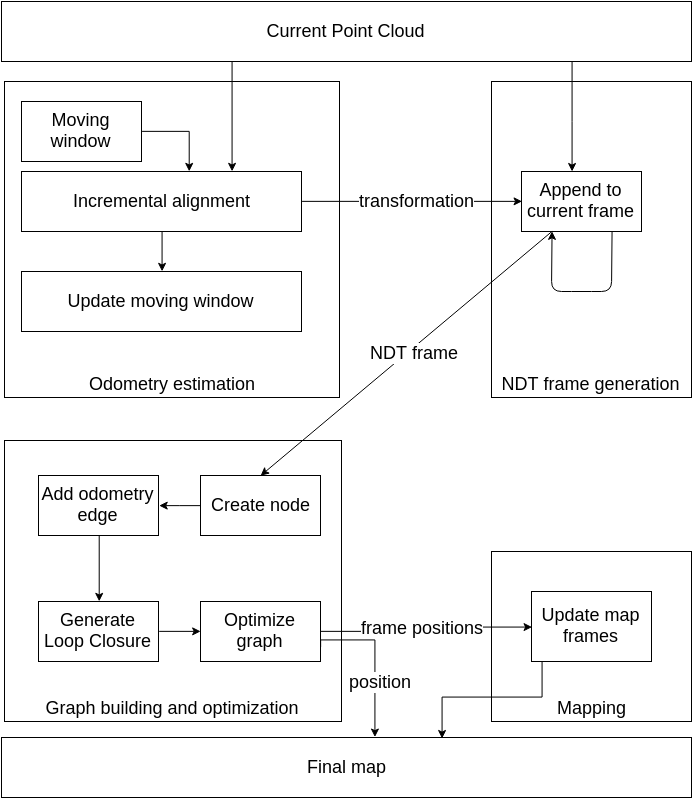
\includegraphics[width=100mm]{../img/algorithm_runtime.png}
	\caption{Diagram of graph based SLAM on NDT maps}
	\label{fig:algorithm}
\end{figure}
  
\newpage


\section{Moving window}
\label{sec:window}
Moving window is a special type of \gls{NDT} grid. It uses all features of \gls{NDT-OM} including occupancy update and dynamic object rejection. Main idea behind moving window is to offer small map which can be used by incremental scanmatcher in order to efficiently align incoming scans against longer history. In standard incremental scanmatching approaches we need to know whole map. Information from whole map is used to correct small errors  when revisiting same place. A problem with this method arise when alignment fails. In this case wrongly aligned scan is merged into the map. This creates single environment feature multiple times in the map. This can be wrongly understood by next registration and error might be never corrected. \gls{NDT-OM} can solve some of degeneration be cleaning occupied cells which are on the way between robot position and new measurement. In order for this mechanism to work next alignment scan needs to converge to original correct position. This is very unlikely with already corrupted mapmand standard NDT technics for registrations, which can end up in local optima during scan refinement step.

In our system, we do not need to know whole map of environment because loops closures errors are fixed by graph optimization. We need incremental scanmatcher to provide us good local estimate of robot movement. For this purpose we only need to know the part of environment occupied by current scan. It strongly depends on the type of sensor and environment. In our setup, robot operated in indoor environment with laser sensor ranging up to 20m in long corridors. In this scenario window size of 20m should incorporate all information which can help in scan registration. If it is possible to select smaller window size based on environment structure this adds to additional speed  and memory efficiency. 

The mowing window also needs to follow movement of the robot to incorporate new measurements. This can be done in two ways. First we might rotate window based on exact changes of robot global position. By doing this we need to transfer whole window  after each small movement of robot. This approach tries to transform every single normal distribution inside grid in every step of algorithm. Transformed cell's distribution may suddenly overlap multiple fields. We would need to develop mechanism how to split original distributions into multiple cells. Better way is to keep windows orientation fixed and only translate window based on robot's movement. This prevents rotation of distributions in cells, but still suffer from same spiting problem. Solution to this problem is by moving window only in multiples of the grid. This does not affect parameters of normal distribution inside of original grid in order to move whole window. After movement some cells may get out of the scope of current window. These cells are destroyed. This also helps to reduce accumulated error in the window by deleting old corrupted measurement. 

To minimize any alignment issues we decided to perform fast scan matching. This means process most of the data from laser. High frequency scan matching does not need initial guess because valid result is reasonably close to inital position of source and target measurements. Registration algorithm capable of this performance needs to work in order of milliseconds. Two algorithms developed for fine registration on top of \gls{NDT} grid are \gls{P2D}-\gls{NDT} and \gls{D2D}-\gls{NDT}. We have decided to use standard \gls{D2D} algorithm, because it offers ten times better run time than \gls{P2D}. Comparative study by \cite{NDTcomparative} shows that even though \gls{P2D} is usually more precise it needs significantly more computation time. Skipping multiple measurements from sensor may cause that we will not be able to robustly estimate transformation and whole process can converge to local minimum. 

\begin{algorithm}
\label{alg:move_window}
    \caption{Moving window processing loop}
\begin{algorithmic}[1]
\Require point cloud $X$
 \Function{calculateTransform}{$X$}
 
 \EndFunction
\end{algorithmic}
\end{algorithm}
\todo{add visualization of running window}

\newpage

\section{NDT frame creation}
\label{sec:NDT_frame}
\gls{NDT} frame is created by merging multiple point clouds based on transformation received from odometry estimation. Important question is how many scans should we combine ? This algorithm uses consecutive addition of transformation as in equation \ref{eq:concat_trans}. Afterwards, it calculates total displacement done by robot. If it is more than threshold we close down old \gls{NDT} frame and start to add scans into new empty frame. A new frame is assigned its coordinate system based on current robot position. Every new scan is transformed into coordinate system of current open frame and merged in. Closed frame is sent to pose graph generation where it is transformed into graph's node.

Selection of good displacement value is important for run of whole algorithm. Small value will create many nodes in pose graph. Every node will reflect only small portion of environment. This will make loop closure computationally expensive by need to evaluate too many possible loop closure nodes. At the same time loop closing algorithm will work with only limited information. This may cause bigger number of local and global ambiguities in registration. A large value of displacement will generate fewer nodes with more information in each node. This is less computationally dependent. On the other hand it creates ambiguous environment inside of \gls{NDT} frame. Loop closure registration may not correctly deduct which part of the same environment in the frame is correct for registering. This forces registration algorithm to correctly identify this situation and solve it. At the same, it wastes optimizer potential for rejection of ambiguous alignments based on topological information of whole environment. 

\section{Loop closure detection}
\label{sec:LoopClosureMetric}
Loop closure detection is done on top of pose graph. Loop detector can use current positions of pose graph's nodes and relative transformations stored in odometry and loop closure edges. With this information we need to find all nodes which can with current node create loop closure edge. The process starts by Dijkstra projection in section \ref{subsec:loop_closure_creation} from current node. During this process algorithm also  calculates relative displacement along edges. Sum of displacements is used as parameter for rejection of nodes which are too close to our current position. These nodes are certainly overlapping with our start node and therefore it is not necessary to check them again. All the nodes passing previous test are used in one of two rejection models. 

First model tests all nodes against selected radius. Second mechanism is using cumulative transformation and covariance calculated by Dijkstra projection. In validating if two nodes overlap we use same metric as presented by \cite{Olson2009Loop}.
\begin{equation}
\varDelta c = (c_{b} - c_{a})
\end{equation}
\begin{equation}
s  = \max(0,\lVert \varDelta c\rVert - r_{a} - r_{b})\frac{\varDelta c}{\lVert \varDelta c\rVert}
\end{equation}
\begin{equation}
mahl = s^{T}P_{a,b}^{-1}s
\end{equation}
where $c_{a}$ and $c_{b}$ are centroids of start and currently compared \gls{NDT} grids; $r_{a}$ and $r_{b}$ are radii of respective \gls{NDT} grids and $P_{a,b}^{-1}$ is inverse of accumulated covariance.
 
Selected nodes are registered by robust \gls{D2D}. Those matches with high score are inserted into the graph. Edges added by this mechanism may still include some errors or ambiguities. Rejection of these edges is done in optimizer.


\section{Robust D2D-NDT registration}
\label{sec:Robust D2D-NDT}
Construction of robust \gls{D2D} registration needs to be fast and precise. In addition, it needs to have a mechanism how to reject invalid association. It also needs to use only information present in \gls{NDT} grids because loop closure mechanism is working only with this data. We knew that \gls{D2D} can offer quick a reliable registration on \gls{NDT} grids with good initial guess. Correlative scan matching algorithm  \ref{subsec:Corr} can provide registration without knowledge of initial guess but in standard version is not possible to operate on top of \gls{NDT} grids. The time performance of this algorithm is also slower than \gls{D2D}. To solve these problems we have developed modified version of correlative algorithm which can work on top of \gls{NDT} grids.

\subsection{Adaptation of correlative registration}
We have started with base algorithm described in section \ref{subsec:Corr}. For our needs it is sufficient when this algorithm provides only rough initial guess. For this reason we use only one layer architecture. Our single grid has cell size double of original size of \gls{NDT} grid. One reason is faster execution time. In first part of algorithm we need to go over large search space. Mainly because we cannot expect any prior information from graph. Larger grid size limits number of translation because we always try translations in multiple of cell size as mentioned in \ref{subsec:Corr}. 

Secondly, we need to transfer original \gls{NDT} grid into reasonable point cloud. In our implementation we have decided to recreate point cloud out of grid by taking mean from every cell with distribution. Colection of these means makes our mean cloud. In addition, we use information about how many points were used to create normal distribution. This information is used in our algorithm as weight for every mean value. Original algorithm uses two point clouds. 

First is called target cloud and is used for creation of look up table. This table is created by projecting all points to individual cells. When is cell occupied by at least one point it is marked with value 1. In our scenario we use cloud of means from target grid to construct look up table. Use of means is more robust to outliers than original look up table from point cloud. Original implementation marked occupied every cell regardless on number of points mapped into it. Our grids needs at least 4 points to create normal distribution. This is limiting influence of single point spread in space and also emphasizing dominant structures in environment. Target grid conversion to mean cloud does not loose any information in comparison to original cloud. This is because look up table and traget grid are aligned. On top of that double step size of look up table makes four cells from target \gls{NDT} contribute to single look up cell.
  
Second source cloud is used for scoring on top of look up table. Every point of point-cloud contributes to total score based on value from look up cell it belongs to. In our case single point represents information about mean center of multiple points. In order to keep all information, algorithm maps mean into correct cell in look up table. By doing this mean only contributed once. Fortunately a score generated by mean can be scaled with use of weight associated with mean. This makes weighted mean point contribute same amount to system as standard points from point cloud. Score function is defined as:
\begin{equation}
score(T,C) = \frac{1}{d}\sum_{p \in C}^{} v(T,p) w(p) 
\end{equation}

where $T$ is transformation which should be applied to point $p$ of cloud $C$. A function $v(T,p)$ applies transformation $T$ to point $p$ maps it to look up table and return score value for single point. A function $w(p)$ return weight of current mean point. Scaling factor $d$ is defined as
\begin{equation}
d = m\sum_{p \in C_{t}}^{}w(p)
\end{equation} 
where $m$ is the maximal value one point can receive from look up table after application of smoothing kernel in equation \ref{eq:smooth_kernel}; $C_{t}$ represents target point cloud. 

Last problem with conversion of source cloud to mean cloud is to handle discretization errors. These errors happen when we need to transform \gls{NDT} grid. In this situation one original \gls{PDF} may overlap multiple cells. A original point cloud would contribute into multiple cells. Our mean formulation would contribute only to one cell based on mean location. To minimize this effect, we map every mean value into the taget look up table which has double cell size in comparison with source \gls{NDT}. This process is similar to multi layer discretization removal in multi layer \gls{NDT} registration \cite{ulas20113d}. Target look up table also include smoothing kernel, which assign some value to cells surrounding occupied cell in table. This also makes mean which could potentially slip out of occupied cell's boundaries contribute into the total score.

By executing these approximations, we were able to create version of correlative estimate on top of \gls{NDT} grids. Coarser resolution improved performance and allowed us search larger search space. Approximation of input cloud into means reduced number of point we need to test in every iteration of algorithm loop. This effectively lowered number of look up table calls, which speeds up whole process. In addition, mean cloud removes outliers from points spread in space.

\subsection{Algorithm overview}
With coarse initial guess estimate we can  constrict whole algorithm. First step is to run on pair of grids correlative estimation algorithm. This offers us the best initial guess it could find in selected search space. In this step we have used coarse look up table. This means that we are still possible almost two \gls{NDT} cell away from right solution. To get right alignment we run \gls{D2D} algorithm. Multi layer definition of \gls{D2D} can converge to right solution if there is one. Problem arise if two matched grids are from diffrent locations and do not share same environment features e.g lines, corners. In this case correlation registration finds the best possible solution, which means that it rotates grid in a way that maximalize score. \gls{D2D} than tryist to find best alignment and usually falss to first local minimum it can find. To solve these situations we propose solution validation process. Example of bad alignment is in figure \ref{fig:bad_align}. 



\subsection{Solution validation}
Robust alignment offers us the best transformation between source and target \gls{NDT} grid. This alignment can fail and do not offer successful registration at all. We need to validate if this registration succeeded or failed. In this algorithm we again use correlative scan matcher. In this case we use cell size of target look up table matching cell size of \gls{NDT} target grid. We map every point from mean source cloud into look up table and receive total score based on contributions of each weighted mean point. In this case discretization is helping us provide better results. In case that some means stay out of target grid it means that registration was less successful which result in lower score. This method is able to reject scans based on their overlap. This method is not able to distinguish wrong alignment in case that two scans look similar but originate in two different parts of environment.

\begin{algorithm}
\label{alg:robust_d2d}
    \caption{Robust \gls{D2D} registration algorithm}
\begin{algorithmic}[1]
\Require source \gls{NDT} grid $G_{s}$ and target \gls{NDT} grid $G_{t}$. Resolution of \gls{NDT} grids $r$. Validation threshold $v$
 \Function{align}{$G_{s}$, $G_{t}$, $r$}
 \State transformation T is identity
 \State ($T$,$score$) $\gets$ correlativeEstimater($G_{s}$, $G_{t}$,$T$, $2*r$)
 \State $T \gets$ alignD2D($G_{s}$, $G_{t}$,$T$)
 \State ($T$,$score$) $\gets$ correlativeEstimater($G_{s}$, $G_{t}$,$T$, $r$)
 \If{$score \geq v$}
	 \State \Return ($T$,$true$) 
 \Else
	 \State \Return ($T$,$false$)
 \EndIf
 \State \Return T 
 \EndFunction
\end{algorithmic}
\end{algorithm}

\begin{figure}
	\centering
	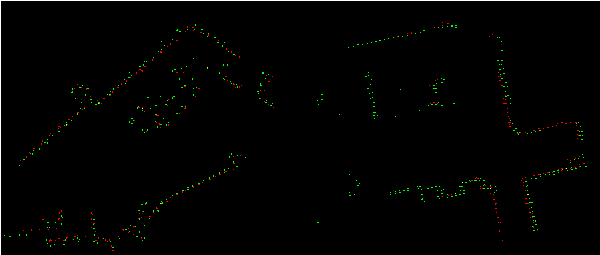
\includegraphics[width=150mm]{../img/good_align.png}
	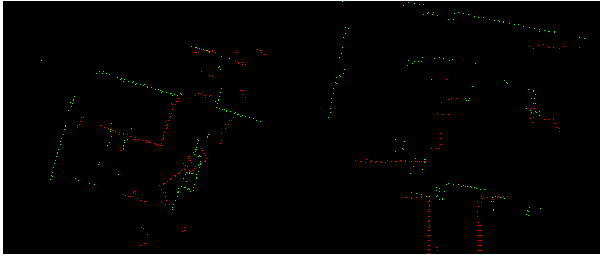
\includegraphics[width=150mm]{../img/bad_align.png}
	\caption{Imiges with alignemt. Red dost represent target scan and green dots source scan. The first row shows valid alignment marked with high score. Second row shows two alignments which were rejected by validation.}
	\label{fig:bad_align}
\end{figure}
  
\subsection{Results}
\newpage

\newpage

\chapter{Implementation}
In this chapter, we will present implementation details of our system. First, we present all libraries used in this project. Later we will introduce outcome in the form of the \gls{ROS} package. Also, we will briefly present the structure of the program and key components.
\section{Used libraries}
\subsection {\gls{ROS}}
The \gls{ROS} \cite{ros_papper} is a popular robotic framework. It offers a flexible way how to combine existing tools, libraries, and algorithms to make a full robotic solution from drivers up to the higher logic of planning and mapping. The communication between individual programs (nodes) is done through the subscriber-publisher model. A configuration of programs is stored in the parameter server. This server also takes care of managing communication between nodes. 
\subsection{The Point Cloud library}
The \gls{PCL} is a standard \gls{ROS} library for manipulation with point clouds \cite{pcl}. The library includes state-of-the-art algorithms in registration, filtering, segmentation, and feature extraction. It also contains tools for visualization and manipulation with point clouds. In our project, we use mostly point cloud class which is the most basic data structure in the library. We also use registration base class for implementation of our scan matching algorithms. 
\subsection{The G2O}
The G2O is a pose graph optimization library presented by \cite{g2o}. It is currently the most used library for the pose graph optimization. It offers well designed extendable interface which makes it easy to add a new definition of pose graph optimization. New optimization methods often have an implementation for this library. In our program, it is used as main optimization engine for our pose graph.
\subsection{The Eigen}
The Eigen \cite{eigenweb} is a templated C++ library for linear algebra. It includes modules for dense and sparse matrix representations, numerical solvers and transformation representation. This project mostly uses geometry module with affine transformation. We also utilize numerical solvers in our implementation of registration algorithms. We have selected this library because it is considered a standard library for linear algebra in the \gls{ROS}. Many packages use it and offer API's designed with this library.   

\section{Structure of the implementation}
 The architecture of the whole system can be divided into three parts. The first part is the\gls{ROS} interface. In our implementation, this interface expects only laser scanner data. However, it is also possible to provide odometry information.  The interface uses standard names for topics. This interface includes all inputs and outputs which can be found in other SLAM packages. Additionally, it provides a map in the form of a point cloud. The full documentation of this interface is in Appendix \ref{chap:ndt_gslam_package}.
 
 The second part is the SLAM algorithm interface implemented in C++. It offers the same functionality as the ROS interface. We have decided to have this double interface because it is convenient to use our SLAM also without the \gls{ROS} subscribe-publish interface. It was mainly used for debugging and testing purposes. This interface also offers some flexibility if we decide to do a different version of our algorithm. In this case, we do not have to rewrite node's source code. In this layer of abstraction, we take care of an initial estimation of the odometry and the \gls{NDT} frame building process. A map generation also takes place in this part of the architecture.
 
 Thirds part is graph \gls{SLAM} interface. This interface makes abstraction around graph creation and optimization process. This section is using our custom pose graph implementation. On top of this graph, we developed a loop closure detection and validation. This graph is synchronized with the graph inside of optimization engine G2O. We carry two graphs for the reason of easier switching between different optimization engines in the future. Our graph representation also includes additional information about state and type of the edge. Implementing it into G2O would require rewriting this code with every new optimizer and with every new G2O edge and vertex type.
 
 An important part of the architecture is handling of \gls{NDT} frames. A created frame is stored inside shared pointer. The same pattern is used in \gls{PCL}'s point cloud data type. The shared pointer is then passed to the graph creation process and also to the \gls{NDT} map building process. Nodes of the pose graph include this pointer as their representation of the world. The \gls{NDT} frames in nodes are used for loop closure registration. This means that registration algorithms use the shared pointers in their API as well. This approach is also a standard for registration algorithm in the \gls{PCL} library
 
 \begin{figure}
 	\centering
 	\includegraphics[width=140mm]{../img/architecture.png}
 	\caption{Overview of individual parts of architecture and their relationships.}\label{fig:architecture}
 \end{figure}
      
\subsection{NDTGrid2D}
The NDTGrid2D is the main class for all operations in our approach. It offers basic functionality for grid creation. It can be merged with or without a use of ray-tracing (occupancy update). It is used for dynamic entity update from \gls{NDT-OM}. It also offers grid translation which is needed for the moving window implementation. Another group of functionality is for registration algorithms. They require radius search and k-nearest neighbor search. The odometry estimator also needs to use means from cells. The last group is output format methods. Grid can create a coarser instance of itself. It is also able to be printed to standard console output. We have implemented methods for conversion into our custom type of occupancy and \gls{NDT} map messages. These messages are used only internally and can be transformed into \gls{ROS} variants.

In order to fulfill all these needs implementation of NDTGrid2D is just a higher abstraction layer on top of the VoxelGrid2D. The voxel grid is taking care of memory layout, resizing, element lookup and ray-tracing. The NDTGrid2D has two template parameters. The first parameter is the type of the cell. Grid is initialized from a point cloud, for this reason, it needs to have second template parameter representing a type of the point. The second parameter is standardly used in \gls{PCL} related algorithms.  

Core algorithm logic for merging and updating cells is stored in every cell. This allows developing new cells without any changes to the grid.
\subsection{VoxelGrid2D}
It is a generic grid-like structure with one template parameter. The type used in the template is required to have implemented operator plus and copy assignment. This data structure is intended to use with larger cell types in the sparse environment. Based on these requirements we designed the memorry model. Grid is represented by single vector which holds pointers to cells. In the case of the unoccupied cell, it uses null pointers. The grid is initialized empty with no cells inside. It allows dynamic resizing either manual or automatic based on inputted cells.  It offers base functionality for ray-tracing and radius search. 
\subsection{NDTCell}
The \gls{NDT} cell is the core of all calculations on top of the grid. In case of \gls{NDT-OM} implementation it holds covariance and mean estimation, occupancy update rule and \gls{RCU} update rule for merging of cells with Gaussian inside. In the future experiments we can easily design a new type of the cell with different calculation model and keep NDTGrid2D and the VoxelGrid without modifications.
\subsection{Registration algorithms}
When designing registration algorithms we have decided to use same interface as \gls{PCL}'s registration algorithms. By extension of their base class our programs can be used standard way inside of \gls{PCL}. This makes it easy to use our algorithms alongside \gls{PCL} implementations. It also possible to use all visualization and io tools provided by \gls{PCL}. Our algorithms have option to run in multiple threads which boost their performance on the multi-core processors. 


\chapter{Evaluation}

\section{Datasets}

\section{Results}


\chapter*{Conclusion}
\addcontentsline{toc}{chapter}{Conclusion}
\gls{NDT} graph-based \gls{SLAM} algorithm presented in section \ref{sec:Sys_arch} can reliably solve localization problem of the robot. It also creates map representation of the world.  The algorithm is suitable for use on robotic systems with a 2D laser scanner. Algorithm does not require odometry information. It is useful especial for robots which do not have any means of providing odometry. The whole process starting with parsing input data and ending with location and map can run in an online matter. The combination of \gls{NDT} scan matcher for fast odometry estimation and pose graph map optimization proven to be a good combination. Correct generation of loop closure was able to save the map from scan matching errors.  Incremental scan matching by itself was not able to correctly map challenging environment. Pose errors were too large. 

The proposed solution to loop closure validation can correctly identify a sufficient number of loop closing constrains. It also offers fast processing time with validation up to 50 loop closures per second. All registration algorithms are implemented with the use of standard \gls{PCL} APIs. It makes them a viable option for use inside of \gls{PCL} ecosystem.

The algorithm is implemented in ROS package ndt\_gslam. This implementation uses a similar interface to other SLAM algorithms in \gls{ROS}.  


%%% Bibliography
%%% Bibliography (literature used as a source)
%%%
%%% We employ bibTeX to construct the bibliography. It processes
%%% citations in the text (e.g., the \cite{...} macro) and looks up
%%% relevant entries in the bibliography.bib file.
%%%
%%% The \bibliographystyle command selects, which style will be used
%%% for references from the text. The argument in curly brackets is
%%% the name of the corresponding style file (*.bst). Both styles
%%% mentioned in this template are included in LaTeX distributions.

\bibliographystyle{plainnat}    %% Author (year)
% \bibliographystyle{unsrt}     %% [number]
%\bibliographystyle{apalike}  
\renewcommand{\bibname}{Bibliography}

%%% Generate the bibliography. Beware that if you cited no works,
%%% the empty list will be omitted completely.

\bibliography{bibliography}

%%% If case you prefer to write the bibliography manually (without bibTeX),
%%% you can use the following. Please follow the ISO 690 standard and
%%% citation conventions of your field of research.

% \begin{thebibliography}{99}
%
% \bibitem{lamport94}
%   {\sc Lamport,} Leslie.
%   \emph{\LaTeX: A Document Preparation System}.
%   2nd edition.
%   Massachusetts: Addison Wesley, 1994.
%   ISBN 0-201-52983-1.
%
% \end{thebibliography}


%%% Figures used in the thesis (consider if this is needed)
\listoffigures

%%% Tables used in the thesis (consider if this is needed)
%%% In mathematical theses, it could be better to move the list of tables to the beginning of the thesis.
\listoftables

%%% Abbreviations used in the thesis, if any, including their explanation
%%% In mathematical theses, it could be better to move the list of abbreviations to the beginning of the thesis.
\chapwithtoc{List of Abbreviations}

%%% Attachments to the bachelor thesis, if any. Each attachment must be
%%% referred to at least once from the text of the thesis. Attachments
%%% are numbered.
%%%
%%% The printed version should preferably contain attachments, which can be
%%% read (additional tables and charts, supplementary text, examples of
%%% program output, etc.). The electronic version is more suited for attachments
%%% which will likely be used in an electronic form rather than read (program
%%% source code, data files, interactive charts, etc.). Electronic attachments
%%% should be uploaded to SIS and optionally also included in the thesis on a~CD/DVD.
\chapwithtoc{Attachments}

\openright
\end{document}
